% article example for classicthesis.sty
\documentclass[10pt,a4paper]{article} % KOMA-Script article scrartcl
\usepackage{import}
\usepackage{xifthen}
\usepackage{pdfpages}
\usepackage{transparent}
\newcommand{\incfig}[1]{%
    \def\svgwidth{\columnwidth}
    \import{./figures/}{#1.pdf_tex}
}
\usepackage{lipsum}     %lorem ipsum text
\usepackage{titlesec}   %Section settings
\usepackage{titling}    %Title settings
\usepackage[margin=10em]{geometry}  %Adjusting margins
\usepackage{setspace}
\usepackage{listings}
\usepackage{amsmath}    %Display equations options
\usepackage{amssymb}    %More symbols
\usepackage{xcolor}     %Color settings
\usepackage{pagecolor}
\usepackage{mdframed}
\usepackage[spanish]{babel}
\usepackage[utf8]{inputenc}
\usepackage{longtable}
\usepackage{multicol}
\usepackage{graphicx}
\graphicspath{ {./Images/} }
\setlength{\columnsep}{1cm}

% ====| color de la pagina y del fondo |==== %
\pagecolor{black}
\color{white}



\begin{document}
    %========================{TITLE}====================%
    \title{{  Notas tema 6 de estadística sobre muestreo aleatorio  }}
    \author{{Rodrigo Castillo}}
    \date{\today}

    \maketitle


     % ====| Loguito |==== %
    
\includegraphics[width=0.1\linewidth]{negro_cara.png}
    %=======================NOTES GOES HERE===================%

    \section{Valores Esperados dela Media Muestal y la Matriz de Covarianza}
        \begin{itemize}
            \item {si las componentes no son independientes o las
                distribuciones no son identicas , la influencia de las medidas
            es asimetrica}
            \item {entonces usamos distancia estadística}
            \item {$ \hat{X}    $  y $ S_n  $  se comportan como estimadores
                puntiales del vector de media poblacional correspondiente y $
            u$ la matriz de covarianza $ \sigma   $  }
        \end{itemize}

        son estimadores \color{brown} blah blah blah \color{white} ...
        \begin{figure}[h!]
            \centering
            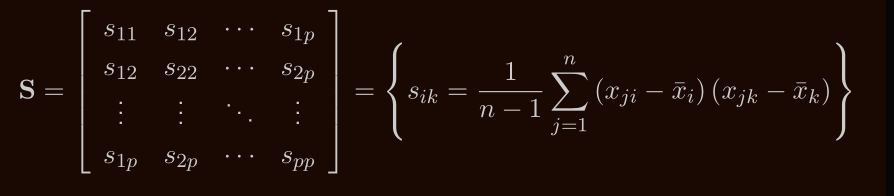
\includegraphics[width=0.8\linewidth]{varianzagen.png}
            \caption{Varianza Generalizada}
            \label{fig:varianzagen}
        \end{figure}

        \color{yellow} nada mas que decir acá \color{white}
        \\


























    %=======================NOTES ENDS HERE===================%

    % bib stuff
    \nocite{*}
    \addtocontents{toc}{{}}
    \addcontentsline{toc}{section}{\refname}
    \bibliographystyle{plain}
    \bibliography{../Bibliography}
\end{document}
